%        File: 26.03.20.tex
%     Created: чт мар 26 08:00  2020 M
% Last Change: чт мар 26 08:00  2020 M
%
\documentclass[algebra,twocolumn]{pum}
\listnumber{4}
\date{26.03.20}
\classname{8-Д}
\lesson{11:30-13:20 }
\tcbuselibrary{raster}
\pgfplotsset{school/.append style={axis lines=middle, xlabel={$x$}, ylabel={$y$}, axis equal, grid=both, xlabel style={at={(ticklabel* cs:1)}, anchor=north west}, ylabel style={at={(ticklabel* cs:1)}, anchor=north west}},graphic/.style={mark=none,thick=8pt,samples=100}}

\begin{document}
\subsubsection*{Определение функций по графику}
Для определения формулы, которая задает функциональную зависимость, по графику это зависимости необходимо сначала определить ту кривую, которая задана графиком. После этого можно пойти одним из двух путей:
\begin{enumerate}
  \item Выписать общий вид функции, график которой построен (в нашем случае это прямая, парабола, гипербола), и по графику в полученное уравнение последовательно подставить столько точек, сколько необходимо для определения неизвестных коэффициентов. Получится система линейных уравнений (опять-таки только в случае рассматриваемых функций) из $n$ уравнений с $n$ неизвестными. 
  \item Определить координаты характерных точек графика функции и попытаться понять с помощью каких преобразований был получен этот график.
\end{enumerate}

Рассмотрим следующий пример:

  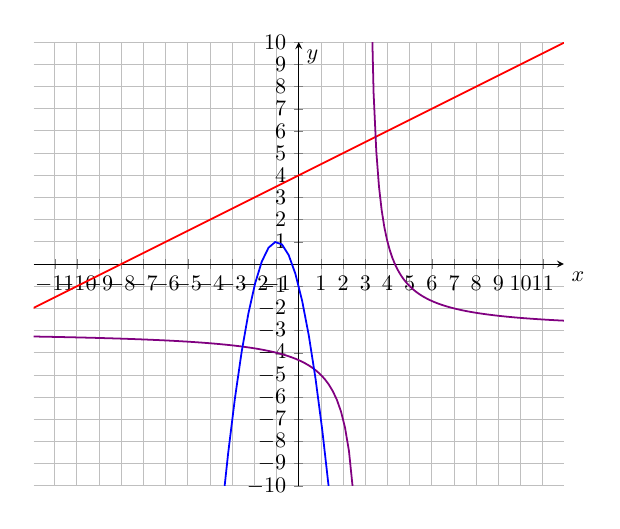
\begin{tikzpicture}[scale=0.8]
    \begin{axis}[
        school,
        width=10cm,
        xmin=-10, xmax=10,
        ymin=-10, ymax=10,
        xtick distance=1,
        ytick distance=1,
      ]
      \addplot[graphic,red,domain=-15:15] {0.5*x+4};
      \addplot[graphic,violet,domain=-15:2.99] {4/(x-3)-3};
      \addplot[graphic,violet,domain=3.01:15] {4/(x-3)-3};
      \addplot[graphic,blue,domain=-15:15] {-2*(x+1)^2+1};
    \end{axis}
  \end{tikzpicture}

  \bigskip
  Красная линия очевидно является прямой. Коэффициент угла наклона положительный, если угол между прямой и осью абсции острый, и отрицательный, если тупой. Отношение модуля ординаты точки пересечения его с осью ординат и модуля абсциссы точки пересечения его с осью абсцисс дает абсолютное значение коэффициента. Чтобы получить красную прямую необходимо график прямой пропорциональности с коэффициентом $k=\frac{1}{2}$ поднять веерх на 4 единицы. Окончательно получаем функцию $y=\frac{1}{2}x+4$, графиком которой является красная линия.
  \bigskip
  \hrule
  \bigskip
  Синяя линяя очевидно является параболой. Ее вершина находится в точке $(-1;1)$.  Парабола сжата, значит коэффициент сжатия больше 1, а именно $2$. Это легко определить, сравнив данную параболу с параболой, вершина которой находится в начале координат. Поскольку ветви параболы направлены вниз, то коэффициент сжатия отрицательный. Окончательно получаем функцию $y=2(x+1)^2+1$, графиком которой является синяя линия.
  \bigskip
  \hrule
  \bigskip
  Фиолетовая линия очевидно является гиперболой. Точка персечения асимптот имеет координаты 3 и -3. Гипербола растянута с коэффициентом растяжения 2. Окончательно получаем функцию $y=\frac{4}{x-3}+3$, графиком которой является фиолетовая линия. 

  \begin{exercises}
    \begin{question}
      Восстановить функцию по графику:

  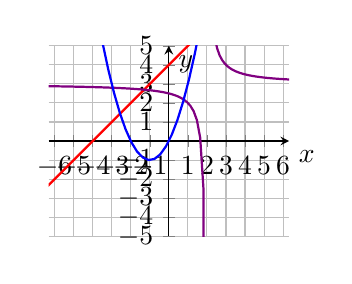
\begin{tikzpicture}
    \begin{axis}[
        school,
        height=4cm,
        xmin=-5, xmax=5,
        ymin=-5, ymax=5,
        xtick distance=1,
        ytick distance=1,
      ]
      \addplot[graphic,red,domain=-15:15] {x+4};
      \addplot[graphic,violet,domain=-15:1.99] {1/(x-2)+3};
      \addplot[graphic,violet,domain=2.01:15] {1/(x-2)+3};
      \addplot[graphic,blue,domain=-15:15] {(x+1)^2-1};
    \end{axis}
  \end{tikzpicture}
    \end{question}
  \end{exercises}

\subsubsection*{Присутствие модуля в функции}
Модуль в формуле, задающей функцию, может обрамлять различные выражения. В двух следующих случаях график функции с модулем может быть получен из графика функции без модуля.
\begin{pumbox}{{$y=f(|x|)$}}
  Зеркально отразить график функции $y=f(x)$ относительно оси {\bf абсцисс}.
\end{pumbox}
\begin{pumbox}{{$y=|f(x)|$}}
  Зеркально отразить график функции $y=f(x)$ относительно оси {\bf ординат}.
\end{pumbox}

\begin{exercises}
  \begin{question}
    Построить графики функций с модулем от $x$:
    \begin{multicols}{2}
      \begin{enumerate}[label=\arabic*)]
        \item $y=|x|$
        \item $y=2|x|$
        \item $y=1-4|x|$
        \item $y=|x|^2$
        \item $y=\frac{1}{2}|x|^2$
        \item $y=-\frac{1}{2}|x|^2-3$
        \item $y=\frac{1}{|x|}$
        \item $y=\frac{1}{4|x|}$
        \item $y=\frac{1}{|x|+4}$
      \end{enumerate}
    \end{multicols}
  \end{question}
  \begin{question}
    Построить графики функций с модулем от функции:
    \begin{multicols}{2}
      \begin{enumerate}[label=\arabic*)]
        \item $y=|2x|$
        \item $y=|2x+3|$
        \item $y=|0.25x-3|$
        \item $y=|0.25(x-4)+2|$
        \item $y=|x^2|$
        \item $y=|x^2-3|$
        \item $y=|(x-1)^2|$
        \item $y=|(x+1)^2+2|$
        \item $y=\left|\frac{1}{x}\right|$
        \item $y=\left|\frac{1}{x}+3\right|$
        \item $y=\left|\frac{1}{x+1}\right|$
        \item $y=\left|\frac{1}{x-2}-5\right|$
      \end{enumerate}
    \end{multicols}
  \end{question}
  \begin{question}
    Построить графики функций с модулем внутри функции:
    \begin{multicols}{2}
      \begin{enumerate}[label=\arabic*)]
        \item $y=2|x-2|$
        \item $y=-|x-2|+3$
        \item $y=|x-2|^2$
        \item $y=|x-2|^2+1$
        \item $y=\left|\frac{1}{x-3}\right|$
        \item $y=\left|\frac{1}{x}\right|+3$
        \item $y=\left|\frac{1}{x+2}\right|-5$
      \end{enumerate}
    \end{multicols}
  \end{question}
\end{exercises}

\end{document}
